\section{Spotify: A Canonical Example} 
For a typical example of a company using many agile teams, consider Spotify who has over 30 teams \cite{kniberg12}.
The basic element of the development organization at Spotify is the Squad, analogous to a Scrum team.
Each Squad is the autonomous developer, with a localized working area, of a particular sub-system in the product.
Squads in related areas are grouped together into Tribes. 
The overall structure is illustrated in Figure~\ref{fig:spotify_structure}.
Although larger than Squads (7-10 members), Tribes are limited in size (< 100) to ensure smooth communication.

\begin{figure}[h]
  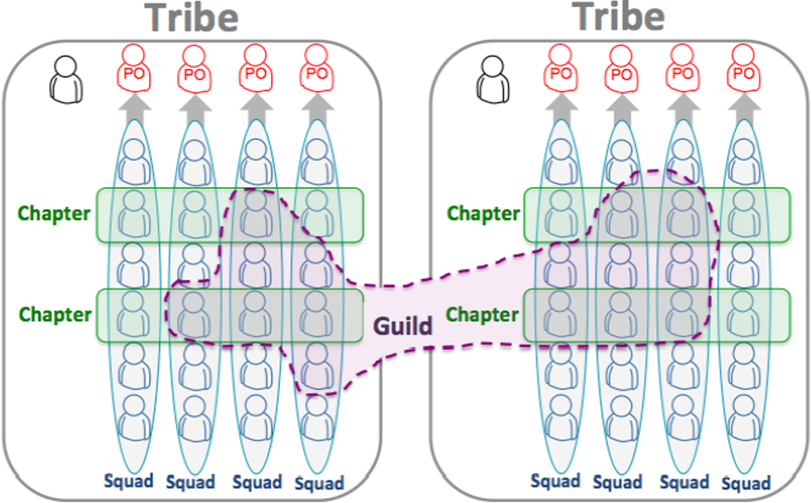
\includegraphics[width=\linewidth]{images/kniberg12_structure.png}
  \caption{Agile team organization at Spotify \cite{kniberg12}.}
  \label{fig:spotify_structure}
\end{figure}


\subsection{Communication}
%social fixes
A fundamental issue with tasking teams with different goals is that teams can become isolated with respect to the context of their work.
At Spotify \cite{kniberg12}, offices are laid out so that the Squads making up a Tribe are spatially close. This leads to an environment where an informal exchange of information on the Tribes work will occur.
%second problem
Consider another scenario: a tester on a particular agile team invests time to solve a particular problem, which is also faced by another tester on a different team. Without communication, these team members would perform redundant work.
To address this problem Spotify defines Chapters \cite{kniberg12}, which are crosscutting divisions which gathers individuals with similar roles across different Squads. 


\section{NAME ME} 

\subsection{Process Improvements} 
\label{sec:proc_impv}
	There are many small changes \cite{collabAcrossAgile_article} that we can incorporate in our process model to make sure that parallel developing agile teams do not run into problems when they reach the integration phase.
	These changes are to be made part of the entire process and are not to be implemented only in the end.

%Changes in standups
	One of the most critical aspect of agile process model is to have daily standups which are the platform serving the purpose of letting each team member know the work being done in the other parts of the team and correlate it with the work being done by them.
	This results in escalation of differences between the development early in the process and prevents end moment discovery of mismatches in interfaces and such.
	In the case of multiple agile teams this problem is compounded as usually a daily stand up is a closed activity of the team itself, thus preventing other teams from knowing the results or discussions of each other.
	This can be resolved by having a representative of each concerned team being present in the daily standup thus letting each team know the status of other teams.

%Changes to Product Owner
Though in usual implementations the product owner is responsible for agile teams under his supervision, in large projects with multiple agile teams where a number of product owners are present sometimes over time the vision of the owners may get too distinct from each other thus pushing the development track in different directions.
This can be limited by having regular meetings of product owners where the scope and vision of the project could be synced again. This can be a bi-weekly or monthly meeting depending on the size of the project.

%Changes in Planning Sessions
All the initial, intermediate and final planning sessions should be made such that all the teams which are or could be impacted by that part of the project are part of the meeting.
This can assist in early agreement on high-level requirements and standardization of inter-team interfaces.

\subsection{Technology Improvements} 
\label{sec:tech_impv}
	A good technology stack can be a powerful tool in maintaining a widely distributed team.
	Good communication and management tools can help the teams in keeping track of things that they need to do so that other teams can work as intended.
	The following are some of the areas where the technology can assist the teams in making a more efficient agile process environment.

%Communication Tools
As agile focuses on personal interaction with highest importance given to face-to-face conversation, conferencing tools such as video conferencing and WebEx etc. can help the team interactions become more fluid and clearer.
They also make the communication real-time thus removing the lag in process due to time spent in communicating ideas across teams.

%Integration Tools
Continuous integration tools can go a long way in finding out inter-team problems early in the process as every time any team makes a change, its impact on the entire project can be seen.

\subsection{Importance of Architecture/Design}\label{sec:imp_of_dsgn}
%Why is Design/Architecture so important when doing this?

As we know that the product owner in an agile process model is the person with the vision of what the project will look like and if it is a small team the product owner can clearly pass this to each and every member of the team and even each member can query the product owner directly when in doubt.
But in large scale projects where multiple agile teams are working together in supervision of a few product owners it is practically impossible for the owner to keep doing what they did in a small team, that’s where a formal definition of their vision comes in handy as it enables the teams to look up to something when encountering a design decision.
The design or architecture in this case acts as a common vision for not only the teams but also for the communication between all the product owners.
The design acts as a “deadlock breaker in decisions” \cite{architecureRole_article} as when the teams can’t come to a common consensus the design shows the path to take.
%non specification fix
Spotify addresses this issue with a more organizational approach by defining a "system owner" role \cite{kniberg12}.
This role is more casual than an architect role, and focuses on defining a "go-to" person who can maintain long term stewardship over a sub-system. 

In addition to specification of system elements, architecture can also be used to empower teams.
As discussed by Parnas \cite{Parnas72}, there are two general approaches to decomposing systems: 1) compartmentalizing a computational process and, 2) focusing on information hiding.
The latter approach ideal for agile development since this approaches defines system components in terms of design dicisions, which empowers invidual teams.